\section{Projektmanagement}

Die Vorgehensweise orientiert sich an Scrum, wird jedoch angepasst auf dieses Projekt.
Scrum ist eine agile, inkrementelle Projektentwicklungsmethode, die oft in der Softwareentwicklung verwendet wird. Dabei wird in Zeitboxen, die Sprint genannt werden, gearbeitet. Pro Sprint gibt es mehrere Tasks, die bearbeitet werden sollen, sowie Sprintziele. Dies wird in diesem Projekt so gemacht.\cite{wikipedia-scrum}

Normalerweise gibt es tägliche Synchronisationsmeetings. Im Rahmen dieses Projektes werden diese wöchentlich durchgeführt, ansonsten wird eher asynchron gearbeitet.

Die Besprechungen der Testatabgaben mit dem Coach dienen als Sprintreviews. Retrospektiven werden nicht strukturiert durchgeführt, jedoch wird zu Ende jedes Sprints besprochen, ob die Arbeitsweise angepasst werden soll für den nächsten Sprint.

Microsoft Teams wird als Scrum Board verwendet. Dies ist ersichtlich auf Abbildung \ref{fig:scrum-board}. Der Backlog wird zu Beginn der Projektes definiert und in einzelne Sprintbacklogs aufgeteilt.

\subsection{Projektorganisation}

Da es sich um eine interdisziplinarische Produktentwicklung handelt, wurde das Team aus jeweils zwei Studierenden aus den Studiengängen Elektrotechnik, Informatik und Maschinentechnik zusammengeführt. In Abbildung \ref{fig:Organigramm} ist die Projektorganisation ersichtlich. 

Im Team wurde Alina Meyer als Projektleiterin gewählt. Zudem benötigt es für die mechanischen und elektrischen Werkstätten in der Hochschule Luzern jeweils eine zuständige Person im Team. Diese wurden Ivan Zimmerman (\acrshort{elektrotechnik}) und Elias von Atzigen (\acrshort{maschinentechnik}) zugeteilt.

Die klare Aufteilung der Rollen ermöglicht es dem Team effizient und zielgerichtet an der Entwicklung des Projekts zu arbeiten. Durch diese Struktur wird gewährleistet, dass jede technische Disziplin angemessen abgedeckt ist und die Kommunikation innerhalb des Teams reibungslos funktioniert.

\begin{figure}[H]
\centering
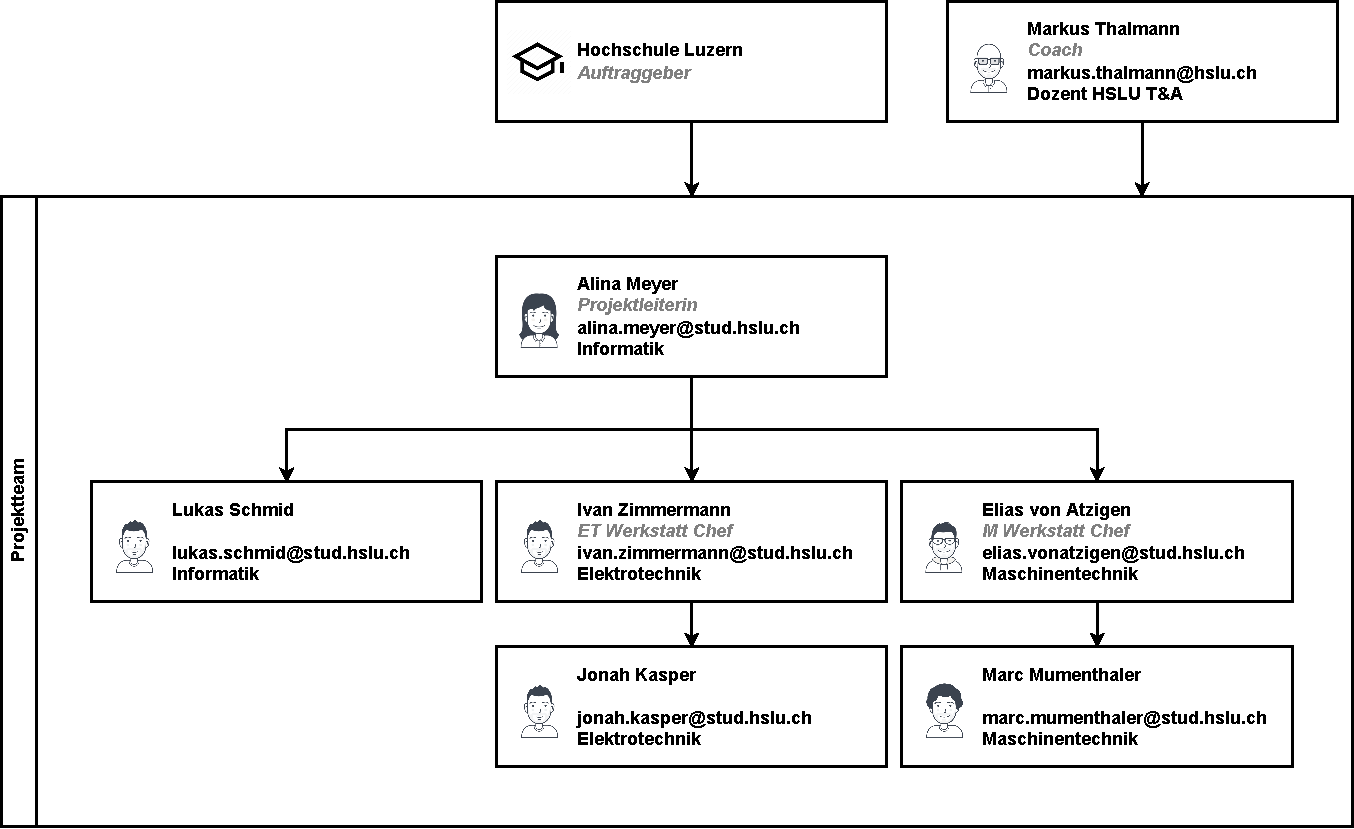
\includegraphics[width=\textwidth]{img/Projektorganisation.pdf}
\caption{Organigramm}
\label{fig:Organigramm}
\end{figure}

\subsection{Datenaustausch}

Zur Zusammenarbeit in diesem Projekt wurde ein Team auf Microsoft Teams erstellt.
Darin ist eine Datenablage, ein Taskboard und ein Chat enthalten. Der Chat wird jedoch weniger verwendet, da die Kommunikation hauptsächlich über WhatsApp erfolgt, damit die Antwortzeiten möglichst kurz sind.

Auf der folgenden Grafik \ref{fig:scrum-board} ist das Scrum Board in Teams ersichtlich. Ebenfalls sind in den Tabs auch die Dateiablage und der Chat sichtbar.

\begin{figure}[H]
\centering
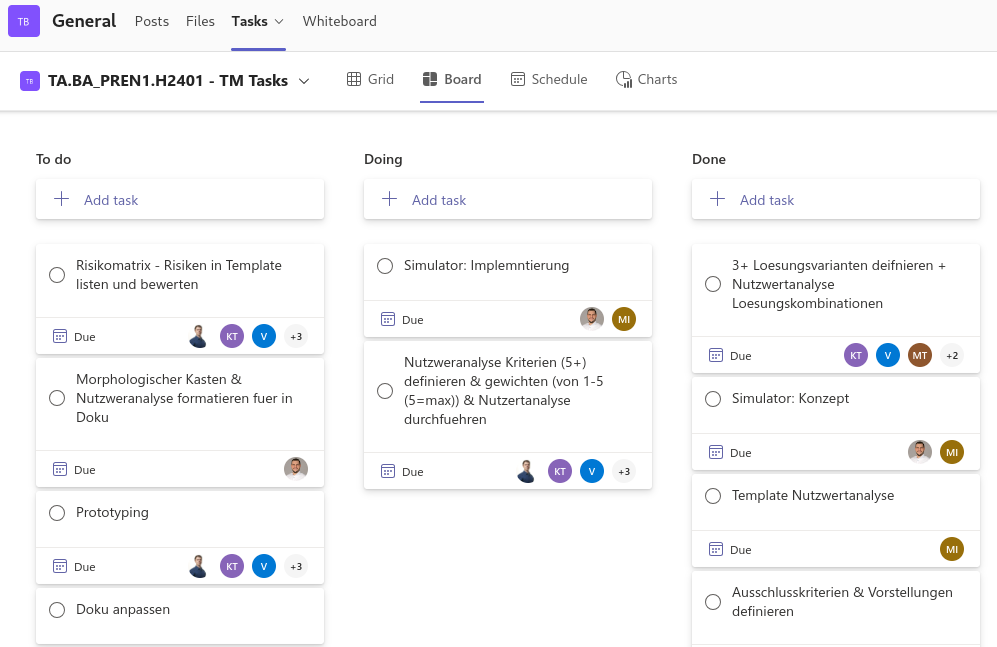
\includegraphics[width=\textwidth]{img/scrum-board.png}
\caption{Scrum Board}
\label{fig:scrum-board}
\end{figure}

Die Dokumentation wird auf einer eigenen Overleaf Instanz in LaTeX erstellt.

Eine detaillierte Auflistung des Datenaustausches und aller Kommunikationsschnittstellen befindet sich im Anhang im Kapitel \ref{kommunikationsplan} Kommunikationsplan.

Der erstellte Code wird auf GitHub gespeichert. Die Planung für den Simulator wird ebenfalls auf GitHub, mithilfe von Issues, durchgeführt. 

Daten aus der CAD Software Siemens NX werden in einem für alle Mitglieder zugänglichen Ordnerverzeichnis auf Teams abgelegt. Die Bauteilbezeichnungen werden in einer separat dafür Vorgesehenen Excel-Datei verwaltet. 

\subsection{Produktkostenkontrolle}

Alle angefallenen Kosten werden laufend gesammelt in einem Ordner auf Teams. Eine Auflistung dieser kann in der Schlussdiskusion im Kapitel \ref{kosten} gefunden werden.

